\subsection{Paket: \pkg{longtable}}

\begin{frame}[fragile]{Das Paket \pkg{longtable}}
\begin{itemize}
\item Tabellen mit Seitenumbruch mit dem Paket \pkg{longtable} erzeugen.\pause
\item Syntax genau wie bei einer normalen Tabelle. \pause
\item Aufruf über die \umg{longtable}-Umgebung. \pause
\item Nachteil: Kann nicht in \umg{table}-Umgebung genutzt werden, da sonst nicht am Ende umgebrochen wird.\pause
\item Arbeit mit der \umg{minipage}-Umgebung: Diese kann innerhalb einer \umg{longtable} auch über mehrere Seiten laufen. 
\end{itemize}
\end{frame}

\begin{frame}[fragile]{hilfreiches Paket: \pkg{longtable}}
\framesubtitle{Beispiel}
\footnotesize
\begin{codeblock}
% benutze das paket fancyvrb
\begin{Verbatim}[fontsize=\tiny]  
\begin{longtable}{|c|c|}
\hline Zeit $t$ & Geschwindigkeit $v_{\text{B}}$  \\ \hline 
\endfirsthead

\multicolumn{2}{c}{Hier gehts weiter...} \\ \hline 
Zeit t & Geschwindigkeit $v_{\text{B}}$  \\ \hline 
\endhead

\hline \multicolumn{2}{|r|}{{Weiter auf der nächsten Seite}} \\ 
\hline
\endfoot

\hline \hline
\endlastfoot

1 & 2 \\ 
 ...
\end{longtable}
\end{Verbatim}
\end{codeblock}
\end{frame}

\begin{frame}[fragile]{\pkg{longtable}(so siehts dann aus)}
\begin{figure}
 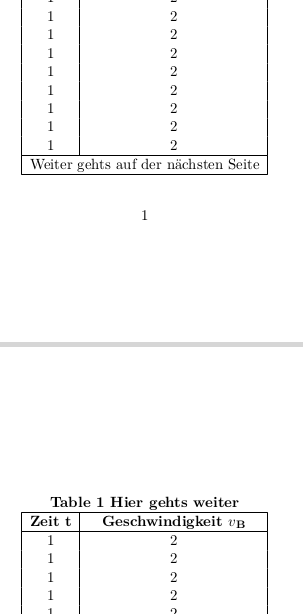
\includegraphics[width=0.3\textwidth]{images/longtable_v2.png}
\end{figure}

\end{frame}

\begin{frame}[fragile]{zu beachten bei \pkg{longtable}}
\begin{itemize}
\item mit \textbackslash endfirsthead definiert man die oberste Zeile der Tabelle 
\item mit \textbackslash endhead definiert man die oberste Zeile der Tabelle auf den folgenden Seiten
\item mit \textbackslash endfoot und \textbackslash endlastfoot analog die letzten Zeilen
\end{itemize}
\end{frame}

